\section{The based cascade: exact residual array and state interface}
\label{ibc:section}

The preceding similarity theorem concerns isolated complete packets.  An
infinite construction cannot be obtained by putting one complete packet after
another.  This section proves the state obstruction, replaces packet reset by
an increment over the retained parent, and calculates the complete normalized
residual of that increment.  The calculation keeps the parent velocity,
velocity gradient, temperature gradient, pressure, buoyancy, diffusion, and
every space-time derivative.

\subsection{A complete packet cannot be reset at the next scale}

The stationary left extension of the complete finite packet has $u=0$.
Hence its vorticity and its origin curl are zero.  At the selected third
return, \eqref{trc:diffusive-root-bounds} gives
\begin{equation}\label{ibc:positive-output-curl}
 2\dot\alpha(T)+\Omega_1(T)+\Omega_2(T)
 \geq \frac{c_W}{4}\sigma_2>0.
\end{equation}
The third vorticity is zero there, so this is the full origin curl of the
three-layer returned state.

\begin{proposition}\label{ibc:reset-obstruction}
No two similarity images of the complete finite packet can be joined in
$C^1$ by identifying the returned endpoint of the first with the stationary
initial endpoint of the second.  This holds for every pair of positive radii,
every pair of positive clocks, and every choice of spatial centre.
\end{proposition}

\begin{proof}
Similarity multiplies vorticity by the positive factor $c^{-1}$, by
\eqref{im:vorticity-scale}.  Thus the returned packet has origin curl at
least $c^{-1}c_W\sigma_2/4>0$.  The stationary initial state of every
complete packet has zero velocity everywhere and therefore zero curl at
every possible centre.  Equality of the first spatial derivatives at a join
would imply equality of their curls.  The strict inequality rules this out.
\end{proof}

The obstruction concerns reset.  The returned state can instead be retained
as the parent of a new increment.  A based cascade performs exactly that
retention.

\subsection{Increment over the full retained parent}

Let $(\theta^{<q},u^{<q},p^{<q})$ solve the equal-diffusion Boussinesq
system with physical diffusion $d>0$ and force
$(f_\theta^{<q},f_u^{<q})$.  Let
$(\vartheta_q,v_q,\pi_q)$ be a smooth increment with
$\operatorname{div}v_q=0$, and set
\begin{equation}\label{ibc:cumulative-state}
 \theta^{[q]}=\theta^{<q}+\vartheta_q,\qquad
 u^{[q]}=u^{<q}+v_q,\qquad
 p^{[q]}=p^{<q}+\pi_q.
\end{equation}

\begin{proposition}\label{ibc:physical-residual}
The state \eqref{ibc:cumulative-state} solves the same equation with force
$(f_\theta^{<q}+e_{\theta,q},f_u^{<q}+e_{u,q})$, where
\begin{align}
 e_{\theta,q}={}&\partial_t\vartheta_q
  +u^{<q}\!\cdot\nabla\vartheta_q
  +v_q\!\cdot\nabla\theta^{<q}
  +v_q\!\cdot\nabla\vartheta_q-d\Delta\vartheta_q,
 \label{ibc:scalar-residual}\\
 e_{u,q}={}&\partial_tv_q+(u^{<q}\!\cdot\nabla)v_q
 +(v_q\!\cdot\nabla)u^{<q}+(v_q\!\cdot\nabla)v_q
 +\nabla\pi_q-d\Delta v_q-\vartheta_qe_2.
 \label{ibc:vector-residual}
\end{align}
\end{proposition}

\begin{proof}
Insert \eqref{ibc:cumulative-state} into both Boussinesq equations.
Subtract the two equations for the parent.  Bilinearity gives the three
displayed transport terms in each row, pressure is additive, diffusion is
linear, and the buoyancy difference is $\vartheta_qe_2$.  Moving that
buoyancy difference to the force side gives the last sign in
\eqref{ibc:vector-residual}.  No parent term remains unlisted.
\end{proof}

Inside the finite construction, each newly activated controlled layer is
multiplied by a switching factor that is flat and zero at its left endpoint.
A future based correction must retain this property for its relative
increment.  The switching factor supplies smooth birth of that increment; it
does not supply the state match calculated below.  Keeping every completed
increment in the parent avoids the reset in
Proposition~\ref{ibc:reset-obstruction}.

\subsection{The normalized parent and the exact scaled residual}

Fix a packet centre $(x_q,t_q)$, radius $\rho_q>0$, and
\begin{equation}\label{ibc:clock}
 c_q=\frac{\delta_*}{d}\rho_q^2,\qquad
 y=\frac{x-x_q}{\rho_q},\qquad
 \tau=\frac{t-t_q}{c_q}.
\end{equation}
Write the increment with the complete similarity weights
\begin{equation}\label{ibc:increment-map}
 \vartheta_q=\frac{\rho_q}{c_q^2}\widetilde\vartheta_q,\qquad
 v_q=\frac{\rho_q}{c_q}\widetilde v_q,\qquad
 \pi_q=\frac{\rho_q^2}{c_q^2}\widetilde\pi_q.
\end{equation}
All tilde fields in this section are evaluated at $(y,\tau)$.  Evaluate the
parent at $(x_q+\rho_qy,t_q+c_q\tau)$ and define
\begin{equation}\label{ibc:parent-map}
 \mathcal U_q=\frac{c_q}{\rho_q}u^{<q},\qquad
 \mathcal D_q=c_q\nabla_xu^{<q},\qquad
 \mathcal G_q=c_q^2\nabla_x\theta^{<q}.
\end{equation}

\begin{proposition}\label{ibc:normalized-residual}
The physical residual increments have the exact form
\begin{equation}\label{ibc:residual-scaling}
 e_{\theta,q}=\frac{\rho_q}{c_q^3}\widetilde e_{\theta,q},
 \qquad
 e_{u,q}=\frac{\rho_q}{c_q^2}\widetilde e_{u,q},
\end{equation}
where
\begin{align}
 \widetilde e_{\theta,q}={}&
 \partial_\tau\widetilde\vartheta_q
 +(\mathcal U_q+\widetilde v_q)\cdot
       \nabla_y\widetilde\vartheta_q
 +\widetilde v_q\cdot\mathcal G_q
 -\delta_*\Delta_y\widetilde\vartheta_q,
 \label{ibc:normalized-scalar}\\
 \widetilde e_{u,q}={}&
 \partial_\tau\widetilde v_q
 +(\mathcal U_q+\widetilde v_q)\cdot\nabla_y\widetilde v_q
 +\mathcal D_q\widetilde v_q+\nabla_y\widetilde\pi_q
 -\delta_*\Delta_y\widetilde v_q
 -\widetilde\vartheta_qe_2.
 \label{ibc:normalized-vector}
\end{align}
Consequently every physical residual jet has exactly the force weights
\eqref{im:force-powers}.
\end{proposition}

\begin{proof}
The time, self-transport, pressure, diffusion, and buoyancy terms have the
common factors already proved in Proposition~\ref{im:similarity}.  For the
parent scalar terms,
\[
 u^{<q}\cdot\nabla_x\vartheta_q
 =\frac{\rho_q}{c_q^3}\mathcal U_q\cdot
       \nabla_y\widetilde\vartheta_q,\qquad
 v_q\cdot\nabla_x\theta^{<q}
 =\frac{\rho_q}{c_q^3}\widetilde v_q\cdot\mathcal G_q.
\]
For momentum,
\[
 (u^{<q}\cdot\nabla_x)v_q
 =\frac{\rho_q}{c_q^2}(\mathcal U_q\cdot\nabla_y)
       \widetilde v_q,\qquad
 (v_q\cdot\nabla_x)u^{<q}
 =\frac{\rho_q}{c_q^2}\mathcal D_q\widetilde v_q.
\]
Substitution proves \eqref{ibc:residual-scaling}--
\eqref{ibc:normalized-vector}.  Differentiating
\eqref{ibc:residual-scaling} gives the last assertion with every space and
time factor retained.
\end{proof}

\subsection{All-order residual arrays}

Let $\alpha=(\gamma_1,\gamma_2,b)\in\mathbb N_0^3$, write
$\partial^\alpha=\partial_{y_1}^{\gamma_1}
\partial_{y_2}^{\gamma_2}\partial_\tau^b$, and define
\[
 \binom\alpha\beta=\prod_{j=1}^3\binom{\alpha_j}{\beta_j},
 \qquad
 (A\star B)_\alpha=\sum_{\beta\leq\alpha}
       \binom\alpha\beta A_\beta B_{\alpha-\beta}.
\]
Let $S_1,S_2,S_t$ shift the corresponding derivative index by one.
Write $S_i^2=S_i\circ S_i$ for the twofold spatial shift.
On the complete normalized support and time interval, set
\begin{align*}
 \mathsf T_\alpha&=\|\partial^\alpha\widetilde\vartheta_q\|_\infty,
 &\mathsf V_{i,\alpha}&=\|\partial^\alpha\widetilde v_{q,i}\|_\infty,
 &\mathsf P_\alpha&=\|\partial^\alpha\widetilde\pi_q\|_\infty,\\
 \mathsf U_{i,\alpha}&=\|\partial^\alpha\mathcal U_{q,i}\|_\infty,
 &\mathsf D_{ki,\alpha}&=\|\partial^\alpha\mathcal D_{q,ki}\|_\infty,
 &\mathsf G_{i,\alpha}&=\|\partial^\alpha\mathcal G_{q,i}\|_\infty.
\end{align*}
Repeated Leibniz differentiation of
\eqref{ibc:normalized-scalar}--\eqref{ibc:normalized-vector} gives the
complete finite majorants
\begin{align}
 \mathsf E^\theta={}&S_t\mathsf T
 +\sum_{i=1}^2(\mathsf U_i+\mathsf V_i)\star S_i\mathsf T
 +\sum_{i=1}^2\mathsf V_i\star\mathsf G_i
 +\delta_*\sum_{i=1}^2S_i^2\mathsf T,
 \label{ibc:scalar-array}\\
 \mathsf E^u_k={}&S_t\mathsf V_k
 +\sum_{i=1}^2(\mathsf U_i+\mathsf V_i)\star S_i\mathsf V_k
 +\sum_{i=1}^2\mathsf D_{ki}\star\mathsf V_i
 +S_k\mathsf P+\delta_*\sum_{i=1}^2S_i^2\mathsf V_k
 +\mathbf1_{k=2}\mathsf T.
 \label{ibc:vector-array}
\end{align}
Thus
\begin{equation}\label{ibc:array-bound}
 \|\partial^\alpha\widetilde e_{\theta,q}\|_\infty
 \leq\mathsf E^\theta_\alpha,\qquad
 \|\partial^\alpha\widetilde e_{u,q,k}\|_\infty
 \leq\mathsf E^u_{k,\alpha}.
\end{equation}
Every parent cross term and every self-interaction appears in these arrays.
These are unsigned majorants, not the signed residual itself.  They give
sufficient estimates but may lose exact pressure, buoyancy, and transport
cancellations.  The correction cycle must reduce the actual residual jets;
a norm of the new field alone is not a force estimate.  The exact signed
array and the failure of a necessary unsigned target are proved in
Section~\ref{irc:section}.

For reference, the parent jets in \eqref{ibc:parent-map} are exactly
\begin{align}
 \partial_y^\gamma\partial_\tau^b\mathcal U_q
 &=\rho_q^{|\gamma|-1}c_q^{b+1}
   (\partial_x^\gamma\partial_t^bu^{<q}),
 \label{ibc:parent-u-jets}\\
 \partial_y^\gamma\partial_\tau^b\mathcal D_q
 &=\rho_q^{|\gamma|}c_q^{b+1}
   (\partial_x^\gamma\partial_t^b\nabla_xu^{<q}),
 \label{ibc:parent-d-jets}\\
 \partial_y^\gamma\partial_\tau^b\mathcal G_q
 &=\rho_q^{|\gamma|}c_q^{b+2}
   (\partial_x^\gamma\partial_t^b\nabla_x\theta^{<q}).
 \label{ibc:parent-g-jets}
\end{align}
With $c_q=(\delta_*/d)\rho_q^2$, their radius powers are respectively
\begin{equation}\label{ibc:parent-radius-powers}
 \rho_q^{|\gamma|+2b+1},\qquad
 \rho_q^{|\gamma|+2b+2},\qquad
 \rho_q^{|\gamma|+2b+4},
\end{equation}
times the displayed fixed powers of $\delta_*/d$ and the corresponding
physical parent derivatives.

\subsection{The state-renormalization equation}

The positive powers in \eqref{ibc:parent-radius-powers} do not permit one
to discard the parent.  The return mechanism requires a nonzero normalized
temperature gradient and a specified normalized velocity gradient.  The
normalized entry profile carried by the retained parent is, by definition,
the triple $(\mathcal U_q,\mathcal D_q,\mathcal G_q)$ in
\eqref{ibc:parent-map}.  For a prescribed next-stage profile
$(\mathcal U_q^{\rm in},\mathcal D_q^{\rm in},
\mathcal G_q^{\rm in})$, equality with that profile is equivalent to the
three exact inverse equations
\begin{equation}\label{ibc:state-interface}
 \begin{aligned}
 u^{<q}(x_q+\rho_qy,t_q+c_q\tau)
    &=\frac{\rho_q}{c_q}\mathcal U_q^{\rm in}(y,\tau),\\
 \nabla_xu^{<q}(x_q+\rho_qy,t_q+c_q\tau)
    &=c_q^{-1}\mathcal D_q^{\rm in}(y,\tau),\\
 \nabla_x\theta^{<q}(x_q+\rho_qy,t_q+c_q\tau)
    &=c_q^{-2}\mathcal G_q^{\rm in}(y,\tau)
 \end{aligned}
\end{equation}
on the required normalized space-time support.  If a proved next-stage entry
set contains more than one such profile, admissibility means that the actual
triple from \eqref{ibc:parent-map} belongs to that set; the inverse equations
remain exact for the profile it realizes.  At the centre, the three physical
scale factors are
\begin{equation}\label{ibc:state-powers}
 \frac d{\delta_*}\rho_q^{-1},\qquad
 \frac d{\delta_*}\rho_q^{-2},\qquad
 \left(\frac d{\delta_*}\right)^2\rho_q^{-4}.
\end{equation}
A parent with uniformly bounded first derivatives tends to zero in the last
two normalized coordinates and cannot reproduce a fixed nonzero entry tuple.
Reproduction of fixed nonzero gradient entries requires the precise
$\rho_q^{-2}$ velocity-gradient and $\rho_q^{-4}$ temperature-gradient
growth encoded by \eqref{ibc:state-interface}.

Equation \eqref{ibc:state-interface} is vector- and matrix-valued.  Choosing
$\rho_q$ from a single norm does not prove it: directions, signs, phase
lengths, parent amplitudes, and every derivative required by
\eqref{ibc:scalar-array}--\eqref{ibc:vector-array} must also match.  The
third-return theorem proves the strict output signs and bounds
\eqref{trc:diffusive-root-bounds}; it does not yet prove that its complete
output, after one dilation, lies in a valid fourth-stage entry set.

This answers the next-step question exactly.  A successful infinite
construction needs a based return-renormalization map satisfying
\eqref{ibc:state-interface}, together with corrections that place the
actual signed residuals \eqref{ibc:normalized-scalar}--
\eqref{ibc:normalized-vector} in the force-flat bounds
\eqref{im:flat-u}--\eqref{im:flat-theta}.  For the concrete choice
$\rho_q=2^{-q}$, bounds
\begin{equation}\label{ibc:target-array}
 \max_{|\alpha|\leq q}
   \|\partial^\alpha\widetilde e_{\theta,q}\|_\infty\leq2^{-q^2},
 \qquad
 \max_{k\in\{1,2\},\ |\alpha|\leq q}
   \|\partial^\alpha\widetilde e_{u,q,k}\|_\infty\leq2^{-q^2}
\end{equation}
are sufficient by the summability calculation following
\eqref{im:explicit-budget}.  The stronger bounds with $\mathsf E$ in
place of the displayed norms are also sufficient, but are not required.
Neither bound is asserted for the present finite packet.  The
complete-copy construction fails
Proposition~\ref{ibc:reset-obstruction}; the based residual and state maps
above are the exact objects that replace it.

The similarity factors, parent-jet powers, residual terms, and convolution
indices are replayed in
\texttt{infinite\_modified/checks/based\_cascade\_check.py}.  Figure~
\ref{ibc:fig:based-cascade} shows the state and force interfaces together.

\begin{figure}[htbp]
 \centering
 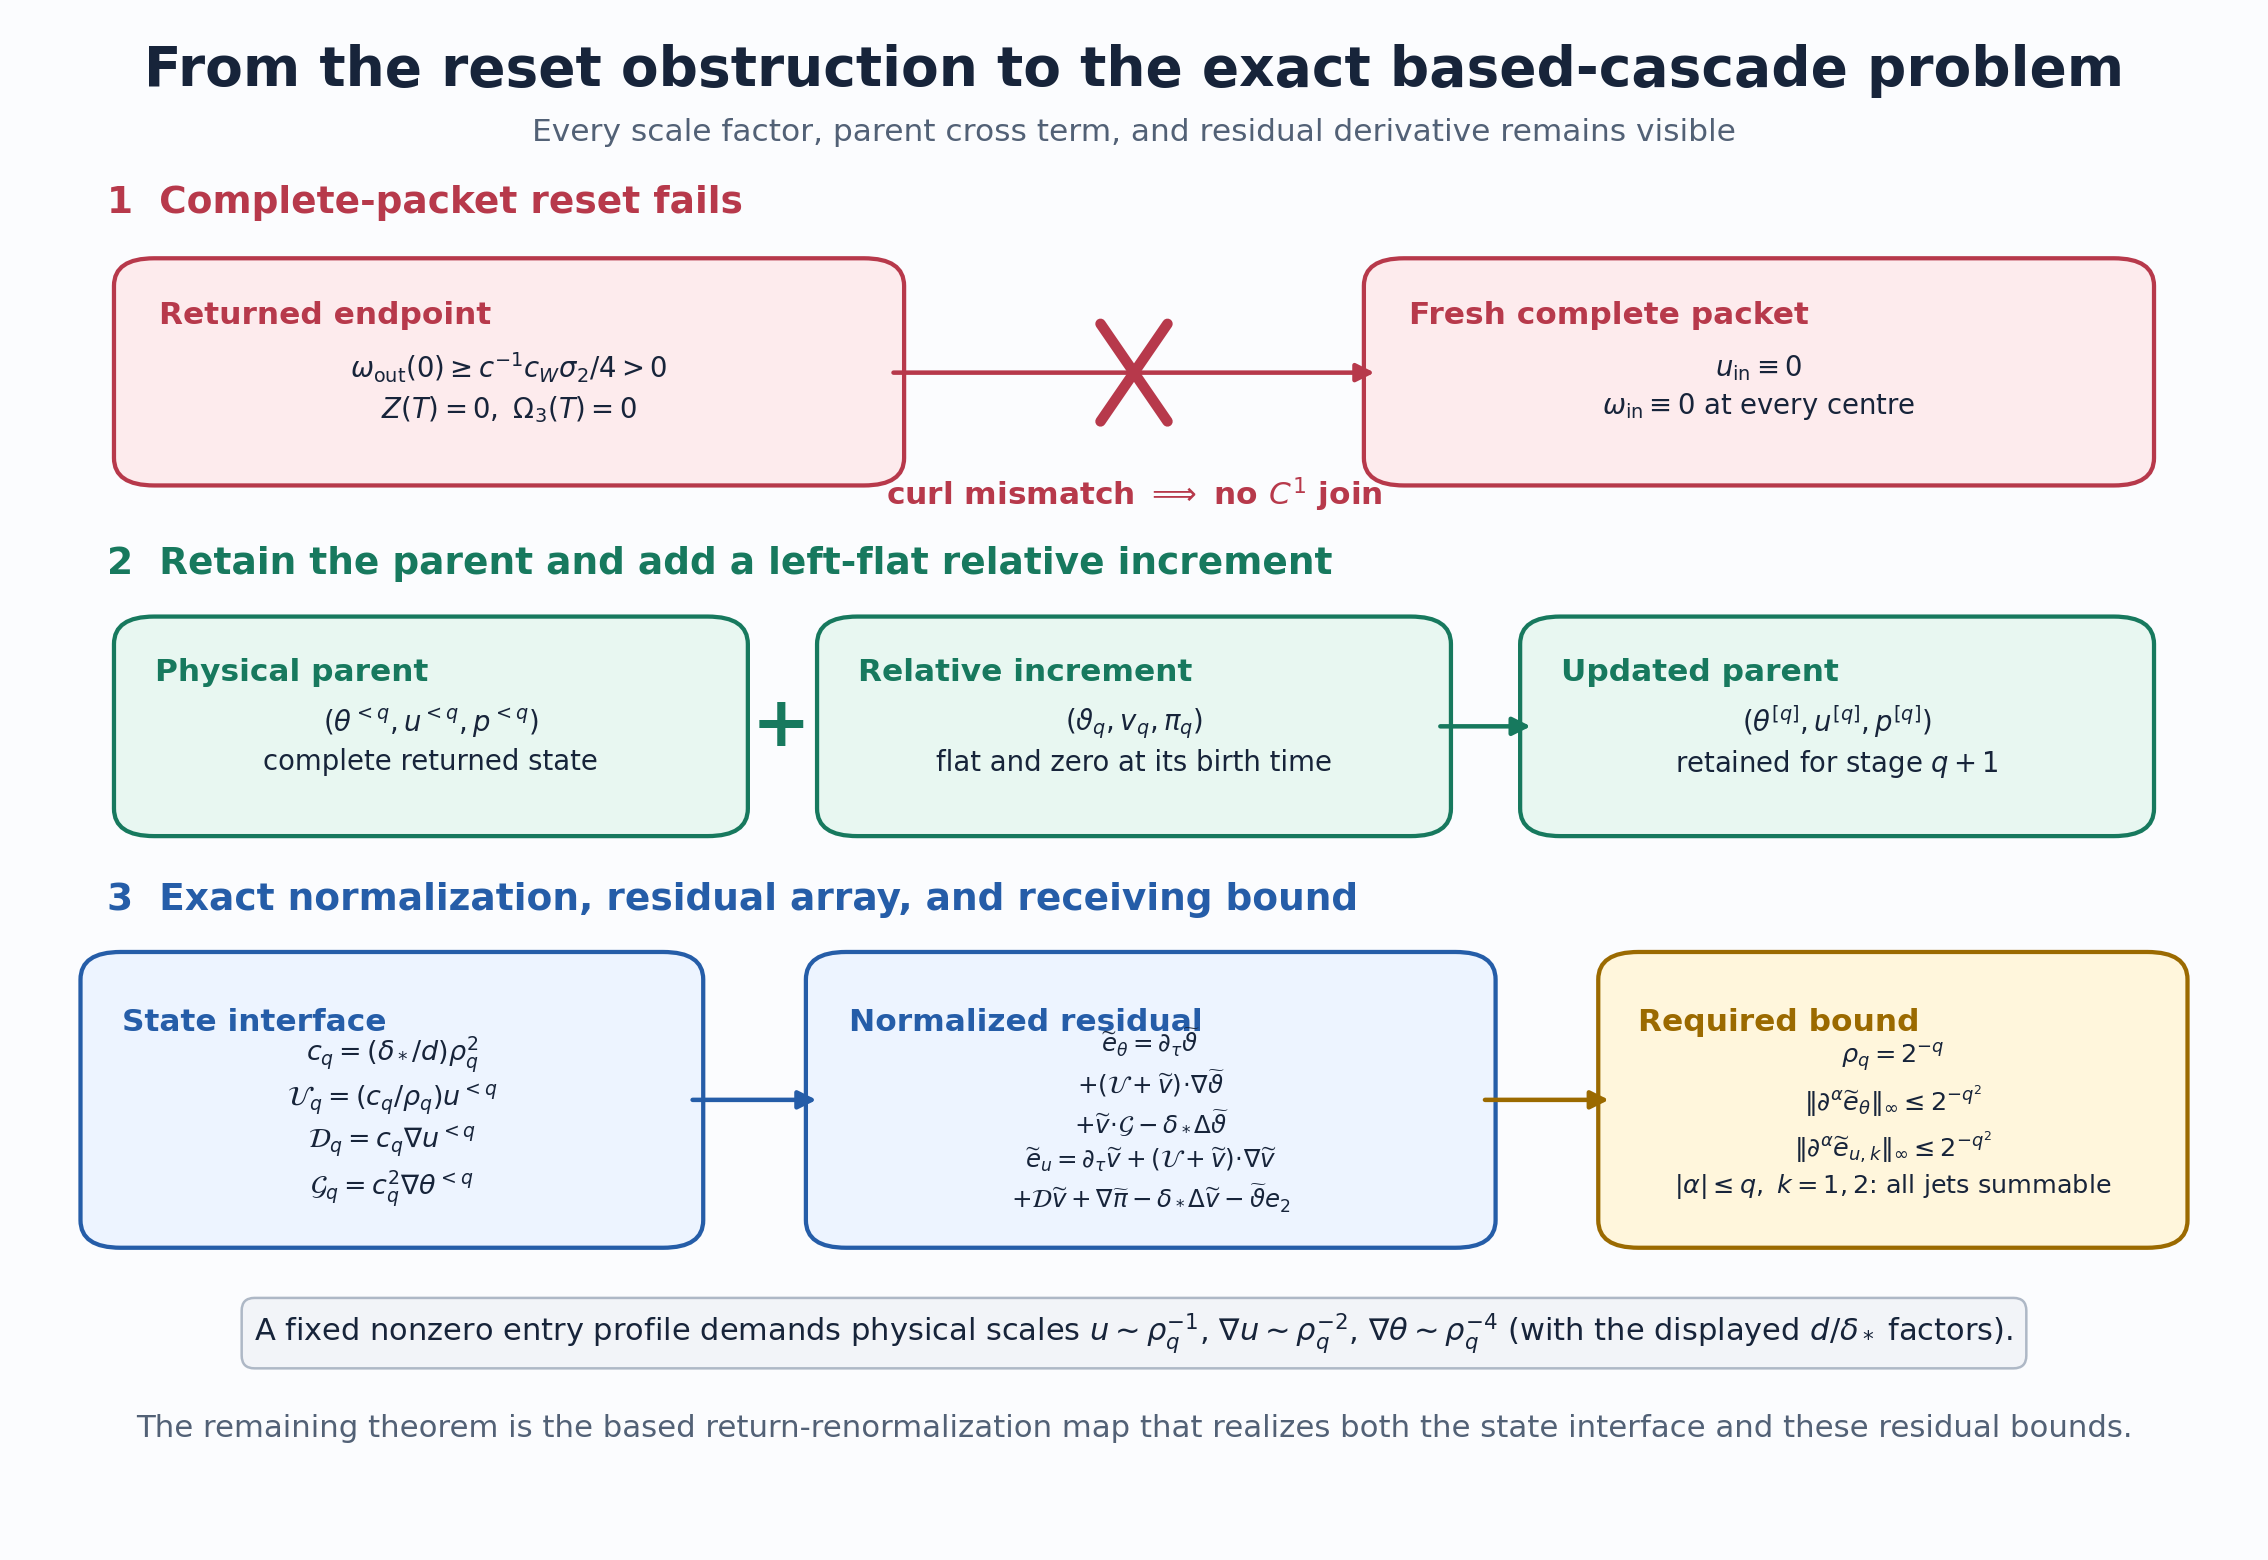
\includegraphics[width=0.96\linewidth]
 {infinite_modified/figures/based_cascade_residual.png}
 \caption{Complete packets fail at the state join because returned curl is
 positive while every reset packet starts with zero curl.  A based cascade
 retains the returned parent, rescales its complete velocity and temperature
 jets through \eqref{ibc:state-interface}, and corrects the exact incremental
 signed residual into the force-flat receiving space.}
 \label{ibc:fig:based-cascade}
\end{figure}
